% benchmark.tex — \input'd from experiments/experiments.tex
%
% Sources: experiments/profiling/benchmark.csv (generated by benchmark.py),
%   experiments/scripts/benchmark.md (analysis writeup).
% Structure: setup, summary statistics, exponential model, practical limits.

\subsection{Performance of EHZ Capacity Computation}
\label{sec:benchmark}

The HK2017 algorithm has exponential cost in the number of facets~$F$.
We benchmark the implementation to establish practical limits for dataset
generation and to quantify the growth rate.

\subsubsection*{Setup}

We generated 76 random 4-polytopes across facet counts~$F = 5, \ldots, 12$
using rejection sampling (seed~42, heights in~$[0.5, 2.0]$), with decreasing
sample counts at higher~$F$: 20 samples at~$F = 5$--$6$, down to 1 sample
at~$F = 12$. Each polytope's EHZ capacity was computed with
\texttt{ehz\_capacity\_pruned} in release mode. Total wall time: 82 seconds.

\subsubsection*{Timing results}

Table~\ref{tab:benchmark-stats} shows summary statistics per facet count.

\begin{table}[h]
\centering
\begin{tabular}{rrrrrr}
\toprule
$F$ & $N$ & Median (ms) & Mean (ms) & Min (ms) & Max (ms) \\
\midrule
 5 & 20 &     1.0 &     1.0 &    1.0 &     1.1 \\
 6 & 20 &     3.7 &     4.0 &    2.4 &     6.7 \\
 7 & 15 &    18.5 &    17.6 &   12.0 &    25.8 \\
 8 & 10 &    83.7 &    88.0 &   59.7 &   159.9 \\
 9 &  5 &   360.5 &   403.7 &  136.2 &   648.3 \\
10 &  3 &  2544.7 &  2114.0 & 1199.6 &  2597.6 \\
11 &  2 & 14775.4 & 14775.4 & 12308.1 & 17242.8 \\
12 &  1 & 42063.3 & 42063.3 & 42063.3 & 42063.3 \\
\bottomrule
\end{tabular}
\caption{EHZ capacity computation time for random 4-polytopes, by facet count.}
\label{tab:benchmark-stats}
\end{table}

\subsubsection*{Exponential model}

A log-linear regression on the median times yields the model
\[
  T(F) \;=\; 3.2 \times 10^{-7} \cdot 4.82^F \quad\text{seconds}
  \qquad (R^2 = 0.997).
\]
The growth rate of~$4.82\times$ per facet is lower than the~$5.74\times$
observed for the five known (symmetric) polytopes in
Table~\ref{tab:validation-results}. This is expected: random adjacency graphs
are sparser than those of highly symmetric polytopes, giving the adjacency
pruning heuristic more branches to cut.

Figure~\ref{fig:benchmark-timing} shows the data and fitted model.

\begin{figure}[h]
\centering
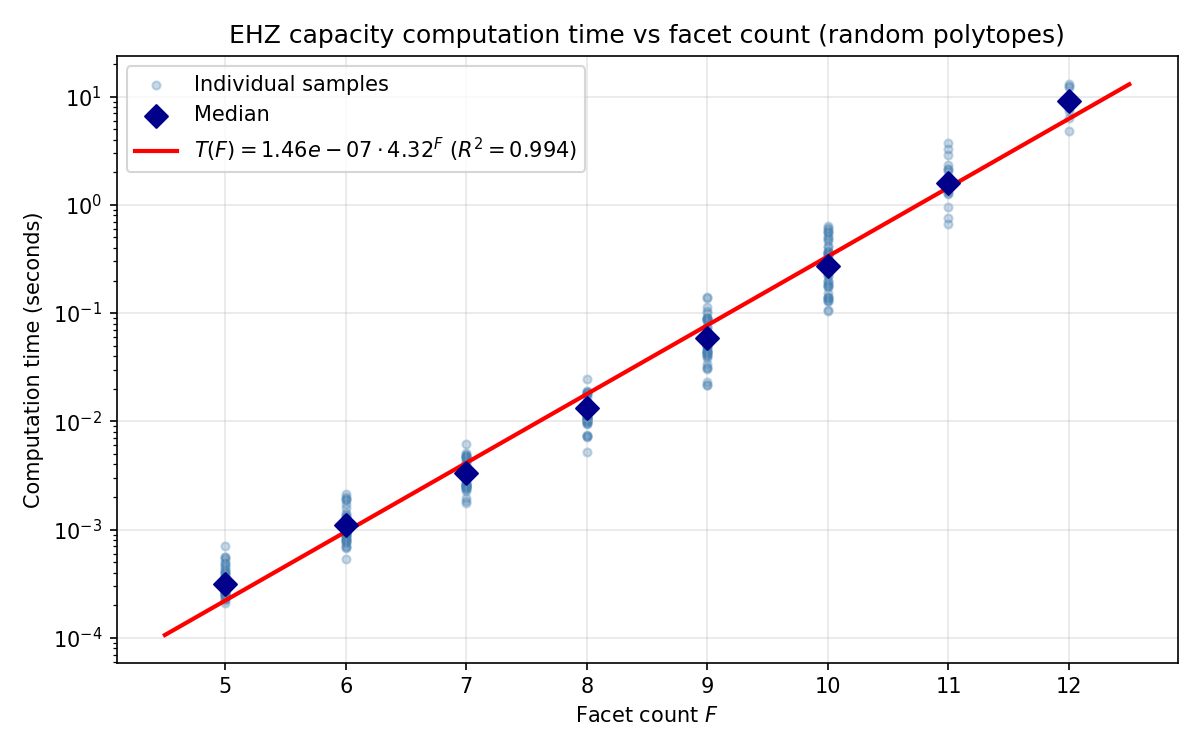
\includegraphics[width=0.75\textwidth]{../experiments/figures/benchmark_timing.png}
\caption{EHZ capacity computation time vs facet count for 76 random polytopes.
  Diamonds: median per facet count. Red line: fitted exponential model.}
\label{fig:benchmark-timing}
\end{figure}

\subsubsection*{Practical limits}

Based on the model:
\begin{itemize}
  \item $F \le 8$: sub-100\,ms, suitable for large datasets (1000+ polytopes).
  \item $F = 9$: $\sim$0.4\,s median, feasible for 50--100 polytopes.
  \item $F = 10$: $\sim$2.5\,s median, feasible for 20--50 polytopes.
  \item $F = 11$: $\sim$15\,s median, feasible for 5--10 polytopes.
  \item $F = 12$: $\sim$42\,s (1 sample), feasible for 1--5 polytopes.
  \item $F = 14$: $\sim$16\,min (projected), single-run only.
  \item $F \ge 15$: hours per polytope.
\end{itemize}

The 16-facet crosspolytope (the smallest known counterexample candidate after
the HK-O pentagon) was tested separately: after 18 minutes, only $m$-levels
2--8 out of 16 were completed, with an estimated total runtime
of~$\sim$400~days. This places the crosspolytope well beyond brute-force reach.
